\documentclass[10pt, UKenglish, xcolor=table]{beamer}
\usepackage{babel}
\usepackage[utf8]{inputenc}  
\usepackage{geometry}
\usepackage[customcolors]{hf-tikz}
\usepackage[T1]{fontenc}   
\usepackage{tcolorbox}
\usepackage{siunitx}
\usepackage{graphicx}
\usepackage{hyperref}
\usepackage{bookmark}
\usepackage{marvosym}
\usepackage{tikz}
\usepackage{tikz-qtree}
\usepackage{cancel}
\usepackage{todonotes}
\useoutertheme[subsection=false]{smoothbars}
\DeclareSIUnit[number-unit-product = {}]{\inchQ}{\textquotedbl}
\usepackage{amsmath}
\usepackage{amssymb}
\newcommand\hmmax{0} % default 3
% \newcommand\bmmax{0} % default 4
\usepackage{bm}
\DeclareSIUnit[number-unit-product = {\thinspace}]{\inch}{in}
\usetheme[menuwidth={0.3\paperwidth}]{erlangen}
\usepackage{multicol}
\usepackage{charter}
\setbeamercovered{transparent=20}
\setbeamertemplate{navigation symbols}{}
\sisetup{separate-uncertainty = true}
%\usepackage[version=4]{mhchem}
\usepackage{tikz}
\usepackage{hepnames}
\usepackage{soul}
\usepackage{color}
\usepackage{thesis_defs}
\usepackage{subcaption}
\captionsetup[subfigure]{labelformat=empty}
\usepackage{xcolor}


\usepackage[backend=biber]{biblatex}
\bibliography{bibliography.bib}

\graphicspath{%
  {./feynman_diagrams/}%
  {./figures_theory/}%
  {./figures_simple/}%
  {./figures_misc/}%
  {./app1/}%
  {./app2/}%
  {./app3/}%
}


\definecolor{color1}{RGB}{33,217,217}
\definecolor{color2}{RGB}{7,61,111}

\newcommand{\lr}{\mathcal{lr}}


\newcounter{totavalue}
\newcounter{parvalue}

\def\aux{1}
\def\radius{9pt}
\def\step{4pt}
\usepackage[absolute,overlay]{textpos}


\newcommand\circcounter{%
\ifnum\inserttotalframenumber<2\relax
\else
  \setcounter{totavalue}{\inserttotalframenumber}
  \setcounter{parvalue}{\insertframenumber}
  \ifnum\inserttotalframenumber>45\relax
    \renewcommand\step{0pt}
  \fi%
  \pgfmathsetmacro{\aux}{360/13}
  \begin{tikzpicture}[remember picture,overlay, rotate=90+\aux]
  \foreach \i in {0,1,...,13}
    \fill[logo_blue] 
      (0,0) -- (-\i*\aux:\radius) arc  (-\i*\aux:-(\i+1)*\aux+\step:\radius) -- cycle;
  \foreach \i in {1,...,\insertframenumber}
    \fill[logo_grey] 
      (0,0) -- (-\i*\aux:\radius) arc  (-\i*\aux:-(\i+1)*\aux+\step:\radius) -- cycle;
  \fill[white] circle (\radius/1.3);
  \node at (0,0) {\small\insertframenumber}; 
  \end{tikzpicture}%
\fi%
}


\usepackage{eso-pic,picture}
\setbeamertemplate{enumerate items}[default]



\begin{document} 

\title[Neural network results in the ditau hadhad channel]{MVA results in the $2\Pe/\Pmu+1\Ptau_{had}$ channel}
\subtitle{\today}
\author{Christian Kirfel, Pablo Martinez Agullo}
%\institute{Universtität Bonn}
        



\begin{frame}[plain]
\vspace{0.0cm}
  \titlepage
      \AddToShipoutPictureFG*{%
    \AtPageUpperLeft{%
      \put(8.7cm,-9.6cm){

\includegraphics[scale=0.03]{original_logo.jpg}
\makebox(0,0)[lt]{}%
      }%
    }%
  }%
    \AddToShipoutPictureFG*{%
    \AtPageUpperLeft{%
      \put(0.0cm,-9.6cm){
%\includegraphics[scale=0.17]{atlas_gay.png}
%
\includegraphics[scale=0.17]{ATLAS-Logo-Ref-RGB-H_0.jpg}
\makebox(0,0)[lt]{}%
      }%
    }%
  }%
\end{frame}
\addtobeamertemplate{navigation symbols}{\vspace*{0.8cm}\hfill\circcounter\hspace*{0.7cm}}

\begin{frame}{Introduction}
  \begin{enumerate}[I]
    \item Summary of MVA methods developed for the dileptau channel
    \vspace{0.3cm}
    \item Explanation of strategies and ongoing efforts
    \vspace{0.3cm}
    \item Comparison of neural network and BDT approaches
    \vspace{0.3cm}
    \item Discussion of future strategy
  \end{enumerate}
\end{frame}

\section*{BDT}


\begin{frame}{BDT Preselection}
    \begin{itemize}
        \item Channel: 2 tight leptons (e/mu) and 1 (hadronic) tau
        \item Region: n-jets $\ge$ 1 and b-jets $\ge$ 1
        \item Significantly decreasing the dominant Z+jets background
        \item Discrepency due to missing tau fake differentiation
    \end{itemize}
    \begin{figure}
        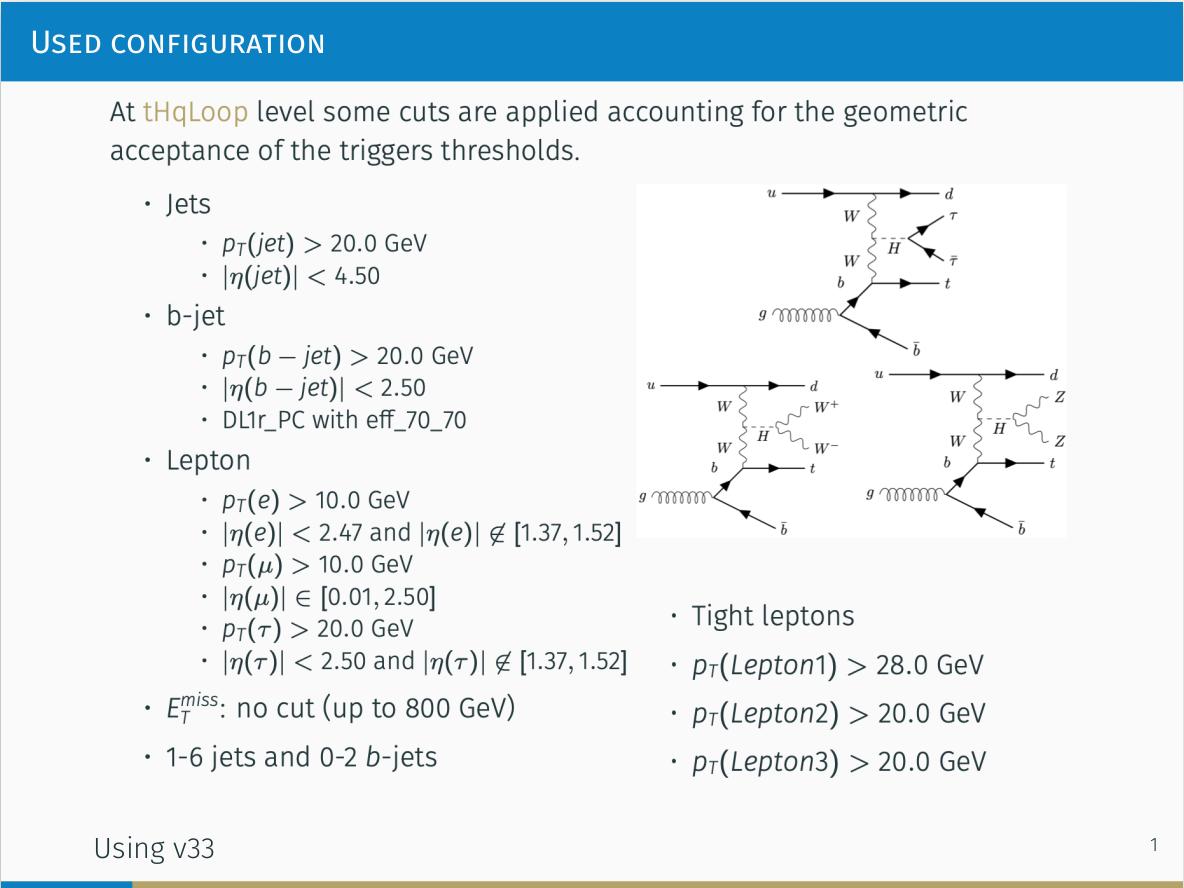
\includegraphics[width=0.7\textwidth]{pablo_selection.png}
    \end{figure}
\end{frame}

\begin{frame}{BDT early results}
    \begin{itemize}
        \item Using XGBoost library
        \item Preliminary: Hyperparameters are not optimised
        \item Visible separation, good training and test agreement
    \end{itemize}
    \begin{columns}
        \begin{column}{0.5\textwidth}
            \begin{figure}
                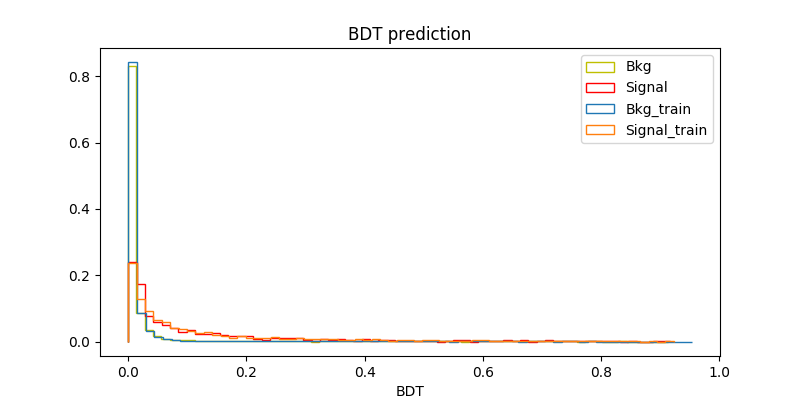
\includegraphics[width=0.9\textwidth]{pablo_response.png}
            \end{figure}           
        \end{column}
        \begin{column}{0.5\textwidth}
            \begin{figure}
                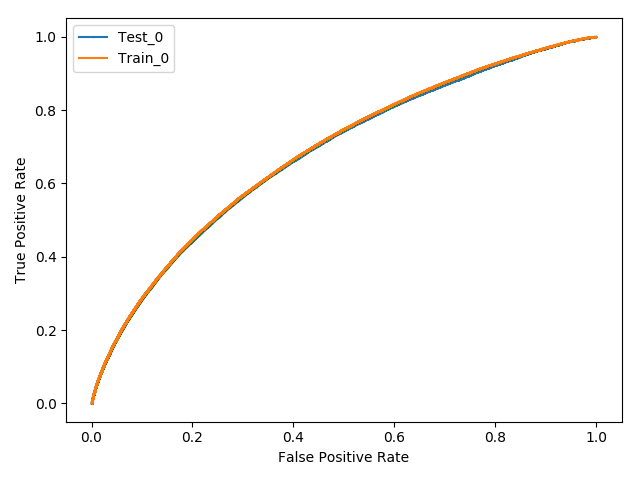
\includegraphics[width=0.9\textwidth]{BDT_ROC.png}
            \end{figure}            
        \end{column}
    \end{columns}

\end{frame}

\begin{frame}{Plan for BDT development}
    \begin{itemize}
        \item {\large BDT hyperparameter tuning}
        \vspace{0.2cm}
        \item {\large Including BDT score in the trees}
        \vspace{0.2cm}
        \item {\large Cut on the BDT score}
        \vspace{0.2cm}
        \item {\large Create a BDT for the CR of the main background}
        \vspace{0.2cm}
        \item Study variables related to SS and OS: Usually, SS and OS have different background contributions.
        \item Get the distributions for forward and central jets separately
    \end{itemize}
\end{frame}
\section*{NN}
\begin{frame}{General ML selection}
    \begin{columns}
      \begin{column}{0.5\textwidth}
        \centering 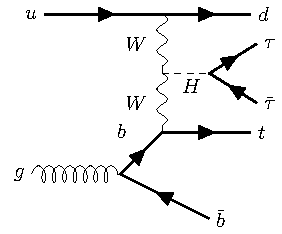
\includegraphics[width=0.8\textwidth]{/cephfs/user/s6chkirf/feynman_diagrams/tHq_tautau}\\
                \begin{itemize}
          \item n-jets: 2 (b-jets: \textbf{1})
          \item b-jet WP: 70 DL1r
          \item nLeptons \& nTaus: $\bf{2e / \mu~1\tau_{\text{had}}} $
          \item $E_{\text{T,miss}}$: no cut (to \SI{800}{GeV})
        \end{itemize}
      \end{column}
      \begin{column}{0.7\textwidth}
        \vspace*{-0.05\textwidth}
        \begin{itemize}
          \footnotesize
          \item jets:
          \vspace*{-0.02\textwidth}
          \begin{itemize}
            \footnotesize
            \item $p_T>\SI{35}{GeV}$
            \item $|\eta|<4.5$
            \item EMPFlow
          \end{itemize}
          \item electrons:
          \vspace*{-0.02\textwidth}
          \begin{itemize}
            \footnotesize
            \item $p_T>\SI{20}{GeV}$ leading \SI{27}{GeV}
            \item $|\eta|<2.5$ not in 1.37 - 1.52
            \item WP: LooseAndBLayerLH ; \\isolation: no requirement
          \end{itemize}
          \item muons:
          \vspace*{-0.02\textwidth}
          \begin{itemize}
            \footnotesize
            \item $p_T>\SI{20}{GeV}$ leading \SI{27}{GeV}
            \item $0.01<|\eta|<2.5$
            \item WP: Loose ; isolation: no requirement
          \end{itemize}
          \item taus:
          \vspace*{-0.02\textwidth}
          \begin{itemize}
            \footnotesize
            \item $p_T>\SI{20}{GeV}$ leading \SI{27}{GeV}
            \item $|\eta|<2.5$ not in 1.37 - 1.52
            \item WP: RNNLoose
            \item ASG recommended OLR ($\tau_{had}$ remove jets)
          \end{itemize}
        \end{itemize}
      \end{column}
    \end{columns}
  \end{frame}


\begin{frame}{Features and weight setup}
  \begin{itemize}
    \item Absolute weights for training because \rightarrow best and most stable results
    \item Preliminary selection of variables
  \end{itemize}
    \begin{columns}
        \begin{column}{0.5\textwidth}
            \resizebox{\linewidth}{!}{
            \begin{tabular}{|l|l|}
                \hline
                eta\_jf          & forward jet eta                        \\ \hline
                pt\_jf           & forward jet transverse momentum        \\ \hline
                mass\_jf         & forward jet mass                       \\ \hline
                phi\_jf          & forward jet phi                        \\ \hline
                eta\_b           & b-jet eta                              \\ \hline
                pt\_b            & b-jet transverse momentum              \\ \hline
                phi\_b           & b-jet phi                              \\ \hline
                HvisMass         & mass of LorentzV sum of hadronic taus  \\ \hline
                m\_met           & Missing energy                         \\ \hline
                Reco\_w\_mass\_2 & Reconstructed mass of the W case 1     \\ \hline
                Reco\_w\_mass\_1 & Reconstructed mass of the W case 2     \\ \hline
            \end{tabular}}
        \end{column}
        \begin{column}{0.5\textwidth}
            \resizebox{\linewidth}{!}{
            \begin{tabular}{|l|l|}
                 \hline
                 deltaRTau        & Delta R of the hadronic taus          \\ \hline
                 deltaPhiTau      & Delta phi of the hadronic taus        \\ \hline
                 HvisPt           & pt of LorentzV sum of hadronic taus      \\ \hline
                 HvisEta          & eta of LorentzV sum of hadronic taus      \\ \hline
                 TvisMass         & mass of reconstructed top             \\ \hline
                 TvisPt           & pt of visible top                     \\ \hline
                 TvisEta          & eta of visible top                    \\ \hline
                 M\_b\_jf         & Mass of LorentV sum of b and jf       \\ \hline
                 HT               & Sum of transverse energies            \\ \hline
                 lep\_Top\_pt     & Light lepton pt                       \\ \hline
                 lep\_Top\_eta    & Light lepton eta                      \\ \hline
             \end{tabular}}
        \end{column}
    \end{columns}
\end{frame}
  


\begin{frame}{Hyperparameters}
  \begin{itemize}
    \item Optimised by small grid search
    \item More thorough optimisation using evolutionary method scheduled, method is in place
  \end{itemize}
    \begin{table}[]
    \begin{tabular}{|l|l|}
    \hline
    Hyperparameter          &     Setting              \\ \hline
    Model                   &     Categorical          \\ \hline
    Nodes                   &     120                  \\ \hline
    Layers                  &     6                    \\ \hline
    Dropout                 &     0.65                 \\ \hline
    Batchnormalisation      &     On                   \\ \hline
    Activation              &     elu                  \\ \hline
    Output activation       &     sigmoid              \\ \hline
    Batch size              &     1000                 \\ \hline
    Optimisation            &     Adam                 \\ \hline
    Weight Initialisation   &     Lecun Normalisation  \\ \hline
    K-folds                 &     4                    \\ \hline
    \end{tabular}
    \end{table}
\end{frame}
  


\begin{frame}{Lephad Features}
    \begin{columns}
        \begin{column}{0.5\textwidth}
            \resizebox{\linewidth}{!}{
            \begin{tabular}{|l|l|}
                \hline
                OSDF\_LepHad            & opposite sign, different flavour                       \\ \hline
                OSSF\_LepHad            & opposite sign, same flavour       \\ \hline
                OS\_LepHad              & opposite sign                      \\ \hline
                OS\_ee                  & opposite sign ee                       \\ \hline
                OS\_emu                 & opposite sign emu                             \\ \hline
                OS\_mue                 & opposite sign mue             \\ \hline
                OS\_mumu                & opposite sign mumu                             \\ \hline
                Reco\_tautau\_mass\_1    & Reconstructed mass of the taus case 1 \\ \hline
                Reco\_tautau\_mass\_2    & Reconstructed mass of the taus case 2                        \\ \hline
                Reco\_w\_Tmass\_1       & Reconstructed transverse mass of the W case 1   \\ \hline
                Reco\_w\_Tmass\_1       & Reconstructed transverse mass of the W case 2     \\ \hline
            \end{tabular}}
        \end{column}
        \begin{column}{0.5\textwidth}
            \resizebox{\linewidth}{!}{
            \begin{tabular}{|l|l|}
                 \hline
                 Reco\_W\_mass\_1      & Reconstructed mass of the w case 1    \\ \hline
                 Reco\_W\_mass\_2      & Reconstructed mass of the w case 2    \\ \hline
                 bscore\_jet1          & bscore jet1          \\ \hline
                 bscore\_jet2          & bscore jet2         \\ \hline
                 m\_met                & Missing energy                \\ \hline
                 vis\_tautau\_mass     & Visible mass of the taus                  \\ \hline
                 vis\_tautau\_pt       & Visible pt of the taus                 \\ \hline
                 vis\_top\_mass\_lep1  & Visible top mass using lepton 1     \\ \hline
                 vis\_top\_mass\_lep2  & Visible top mass using lepton 2  \\ \hline
                 vis\_top\_pt          & Visible pt of the top                             \\ \hline
                 vis\_top\_pt\_lep1    & Visible top pt using lepton 1    \\ \hline
                 vis\_top\_pt\_lep2    & Visible top pt using lepton 2    \\ \hline
             \end{tabular}}
        \end{column}
    \end{columns}
\end{frame}

\begin{frame}{Lephad Hyperparameters}
    \begin{table}[]
    \begin{tabular}{|l|l|}
    \hline
    Hyperparameter          &     Setting               \\ \hline
    Nodes                   &     40                    \\ \hline
    Layers                  &     6                  \\ \hline
    Dropout                 &     0.4                  \\ \hline
    Batchnormalisation       &     On                   \\ \hline
    Activation              &     elu                  \\ \hline
    Output activation       &     sigmoid              \\ \hline
    Batch size              &     150                 \\ \hline
    Optimisation            &     Adam                 \\ \hline
    Weight Initialisation   &     Lecun Normalisation  \\ \hline
    \end{tabular}
    \end{table}
\end{frame}
  
\begin{frame}{Monitoring hadhad}
\begin{columns}
  \begin{column}{0.5\textwidth}
    \begin{figure}
      \includegraphics[width=\textwidth]{losses_lephad.png}
    \end{figure}
  \end{column}
  \begin{column}{0.5\textwidth}
    \begin{figure}
      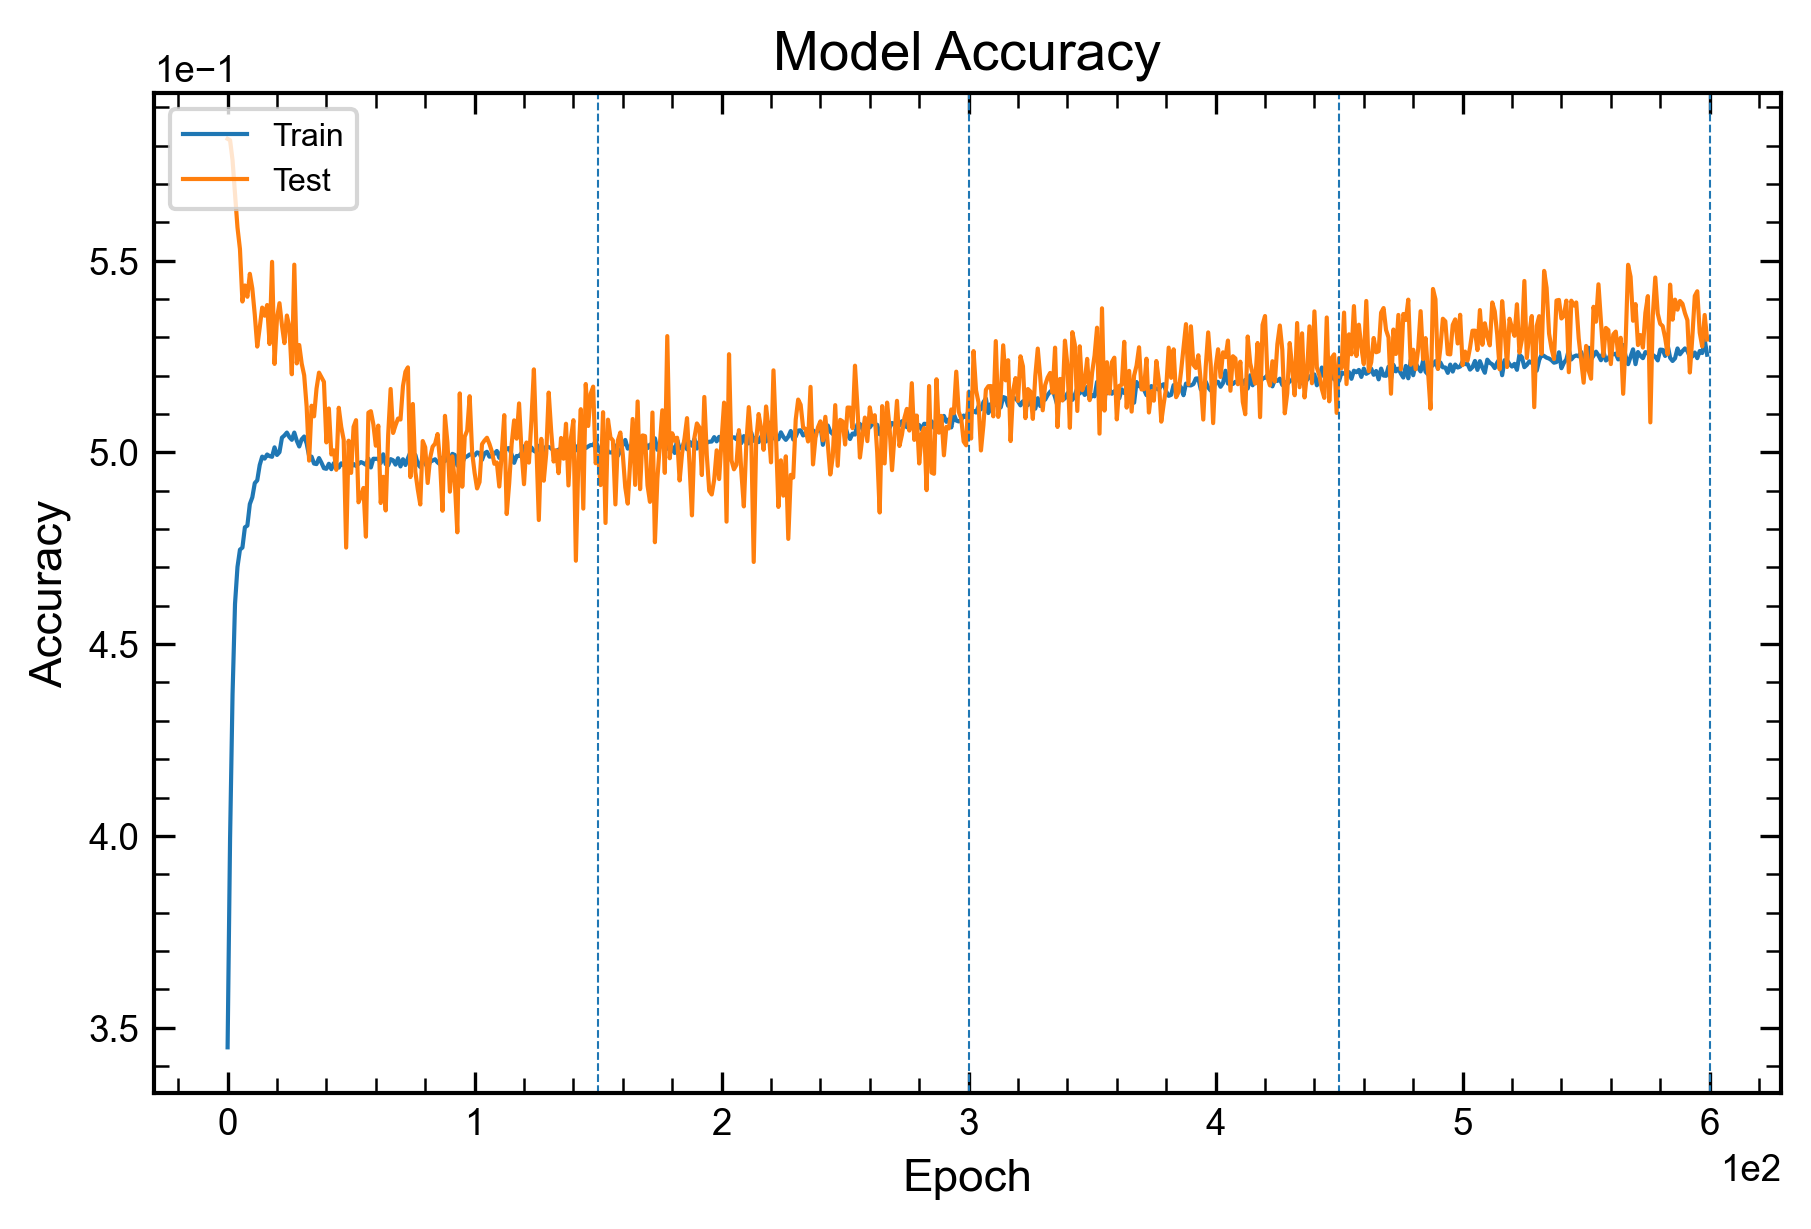
\includegraphics[width=\textwidth]{acc_lephad.png}
    \end{figure}
  \end{column}
\end{columns}
\end{frame}

\begin{frame}{Results hadhad}
\begin{columns}
  \begin{column}{0.5\textwidth}
    \begin{figure}
      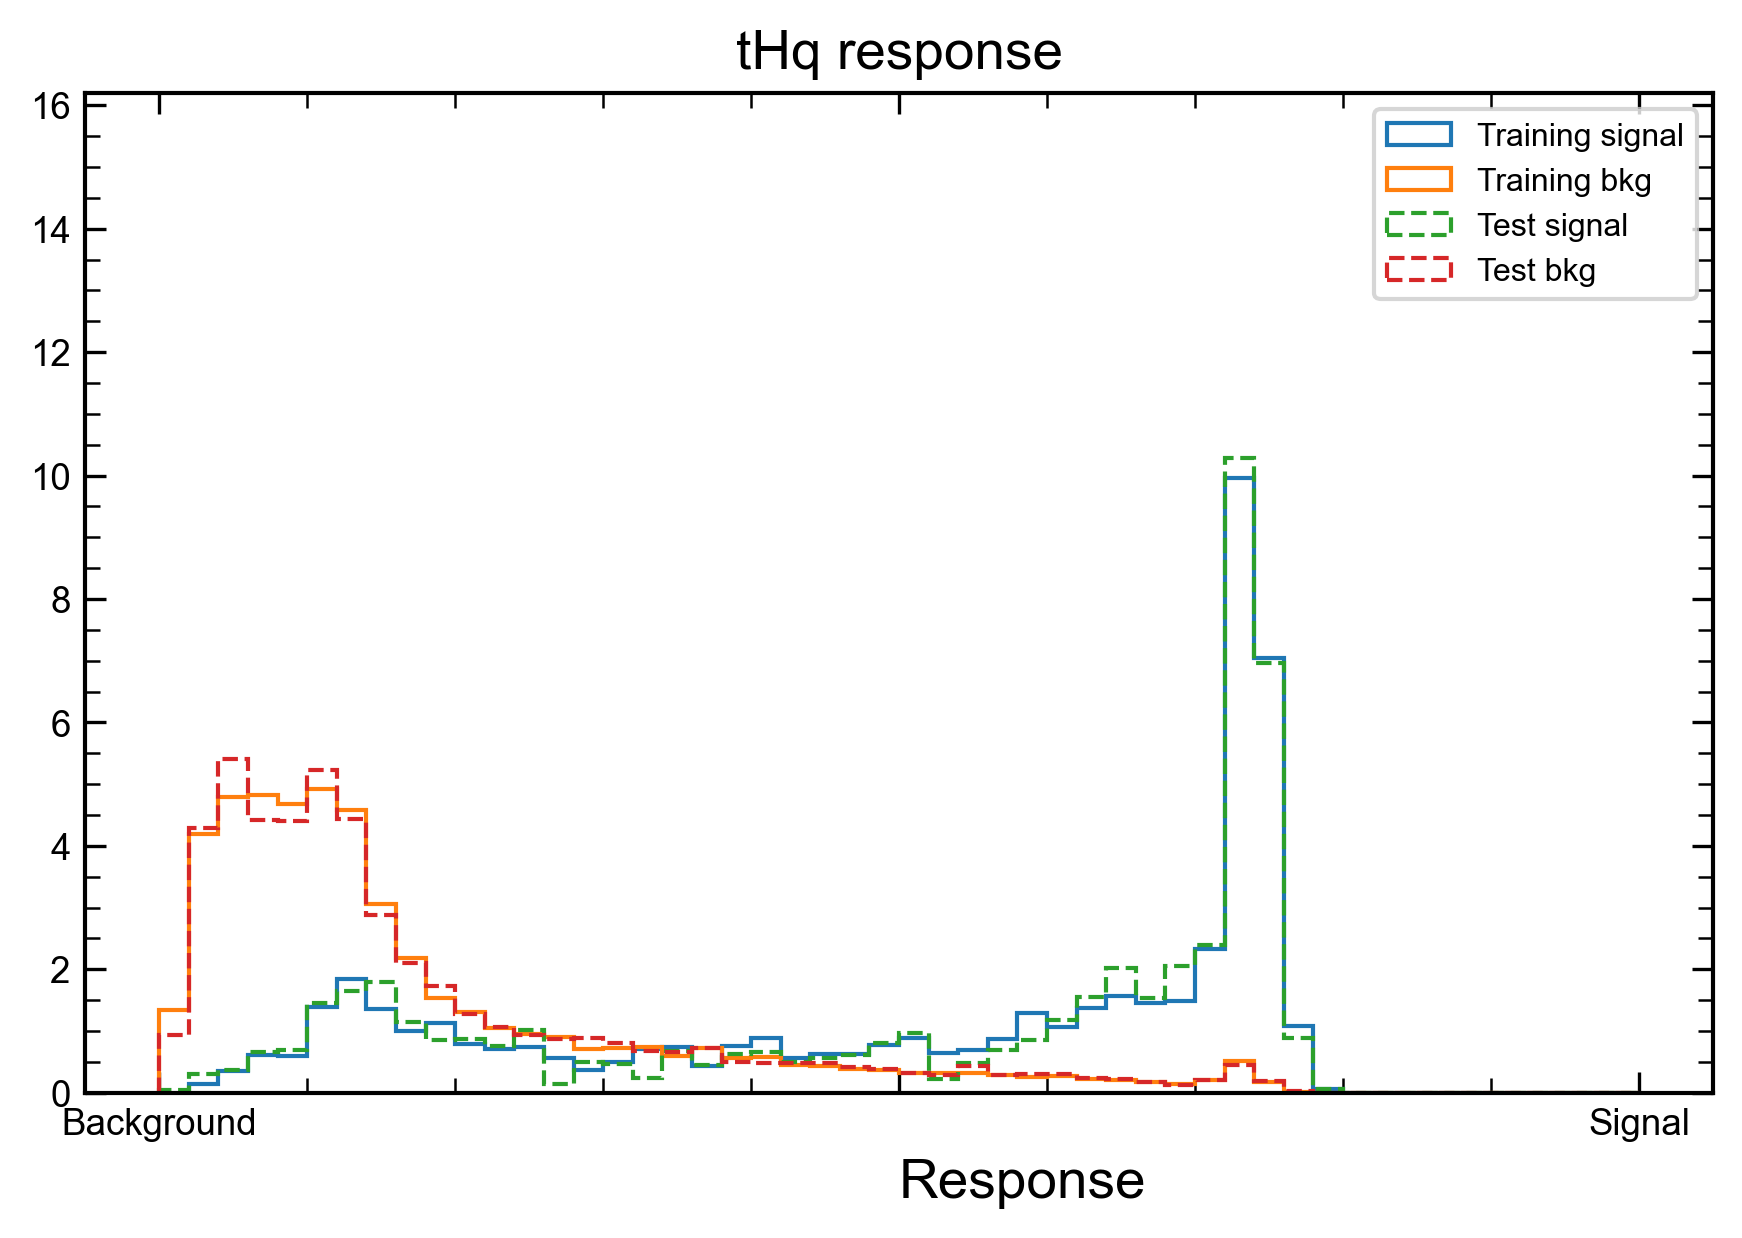
\includegraphics[width=\textwidth]{response_lephad.png}
    \end{figure}
  \end{column}
  \begin{column}{0.5\textwidth}
    \begin{figure}
      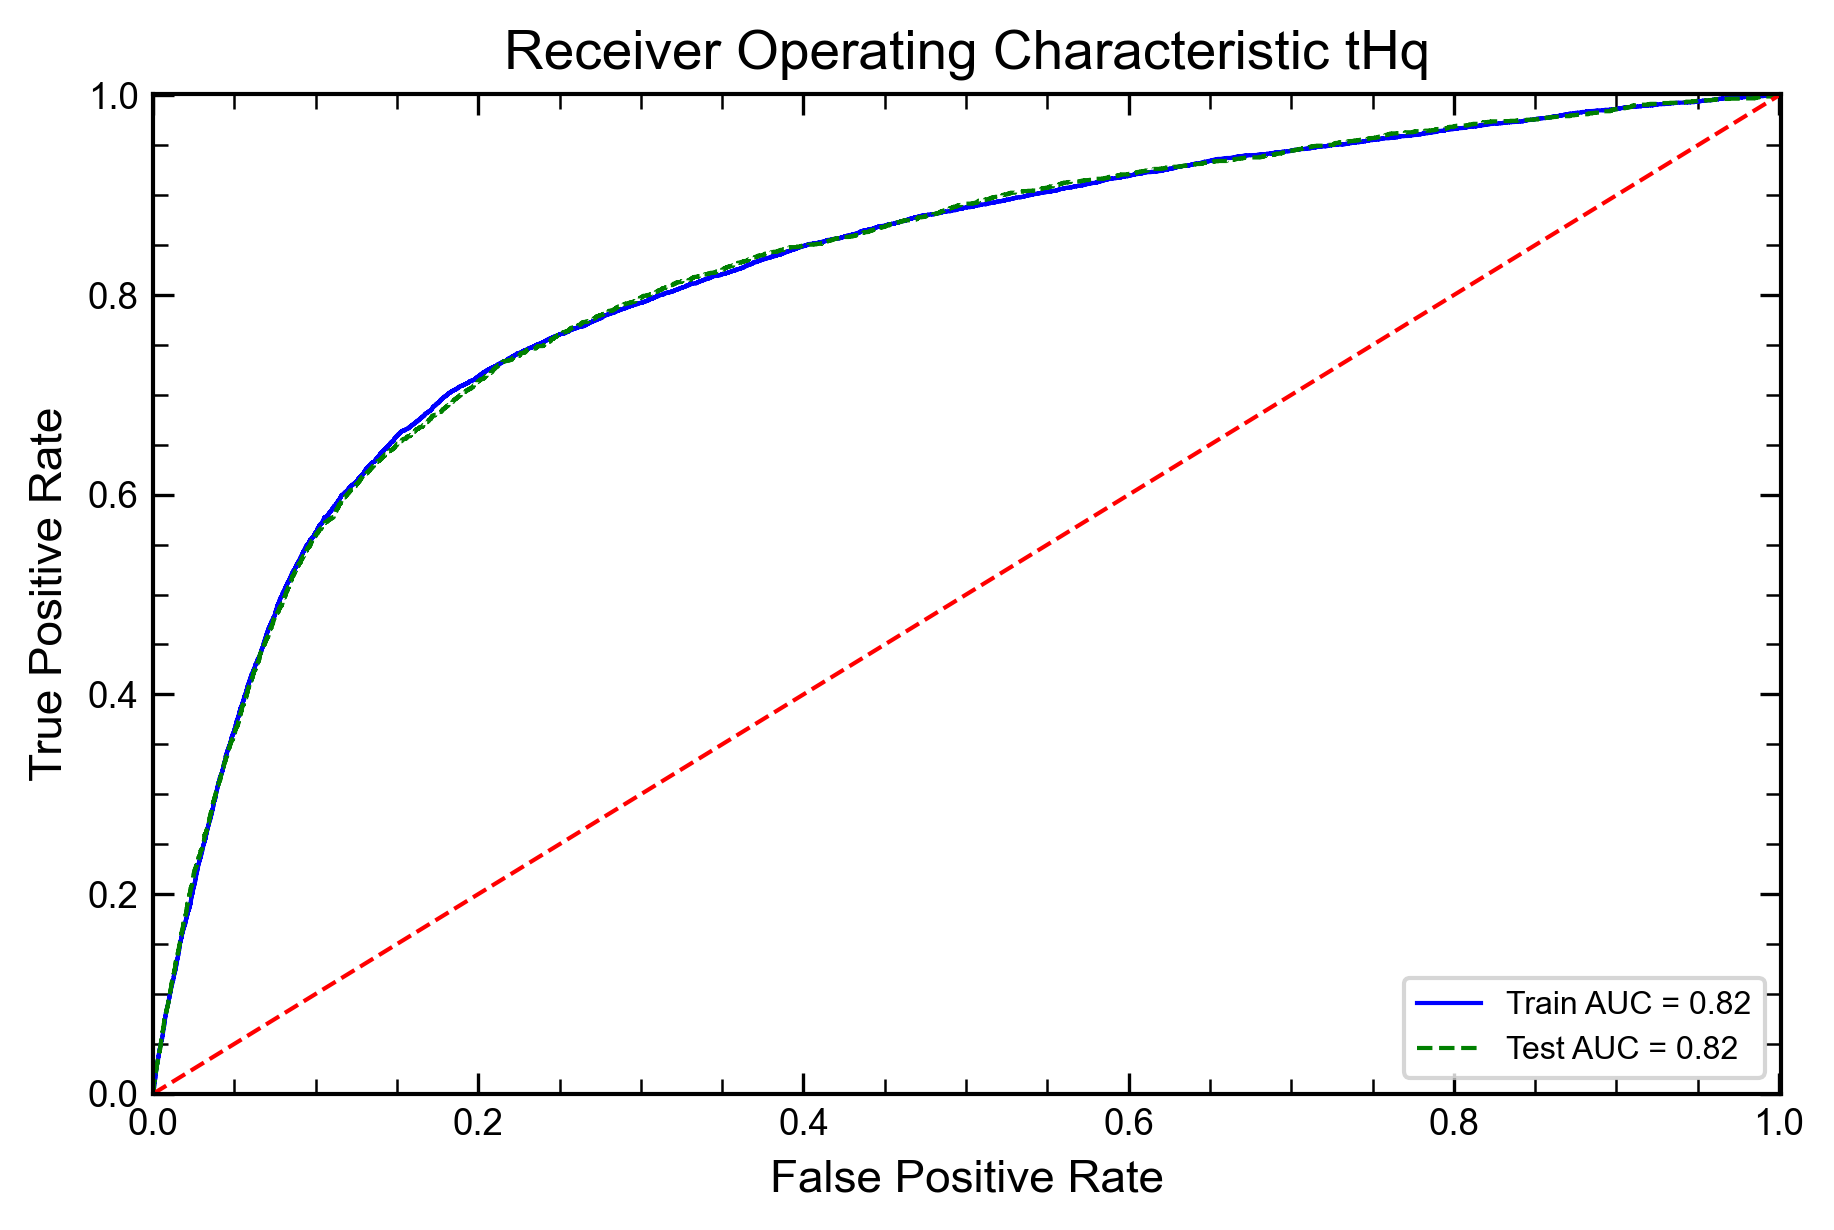
\includegraphics[width=\textwidth]{ROC_lephad.png}
    \end{figure}
  \end{column}
\end{columns}
\end{frame}
\section*{\tZq}


\begin{frame}{Responses}
    \begin{columns}
        \begin{column}{0.5\textwidth}
            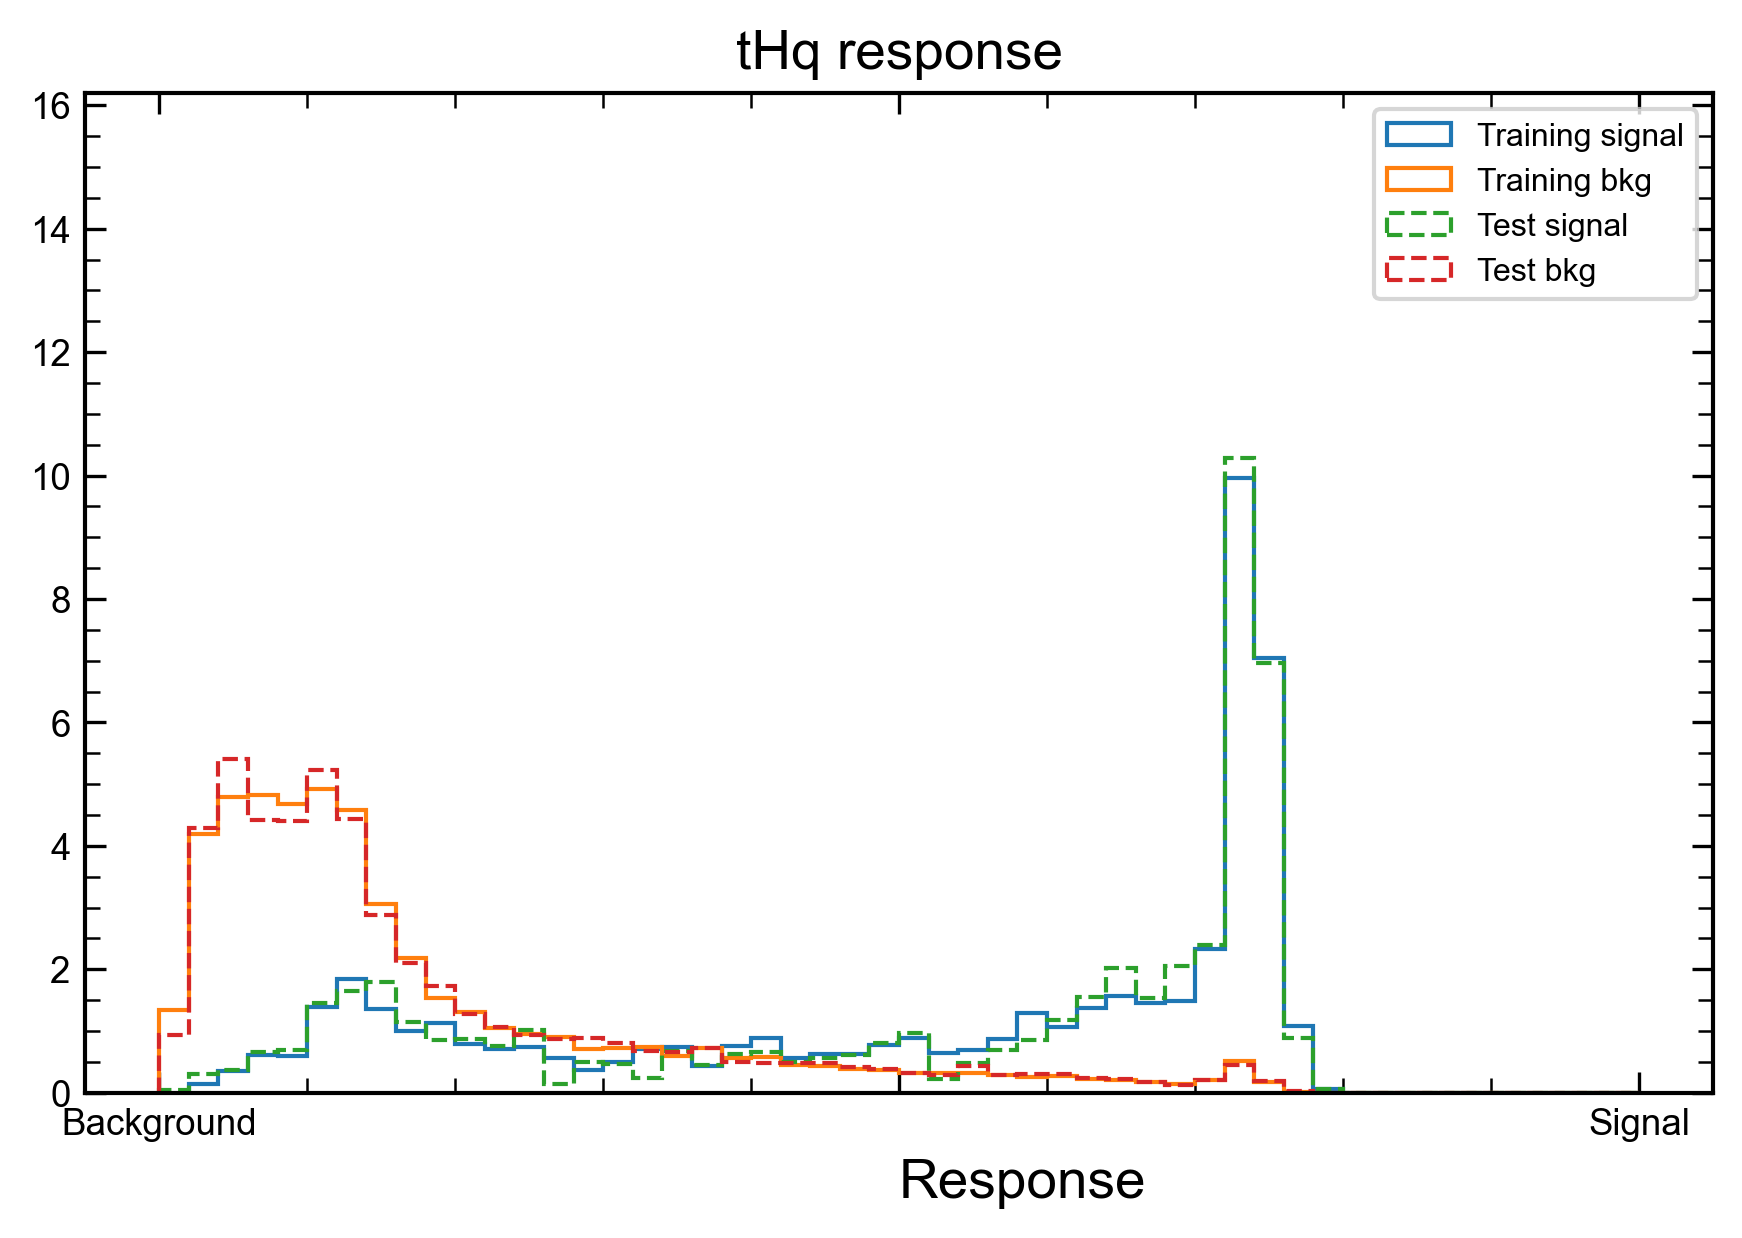
\includegraphics[width=0.8\textwidth]{response_lephad}
            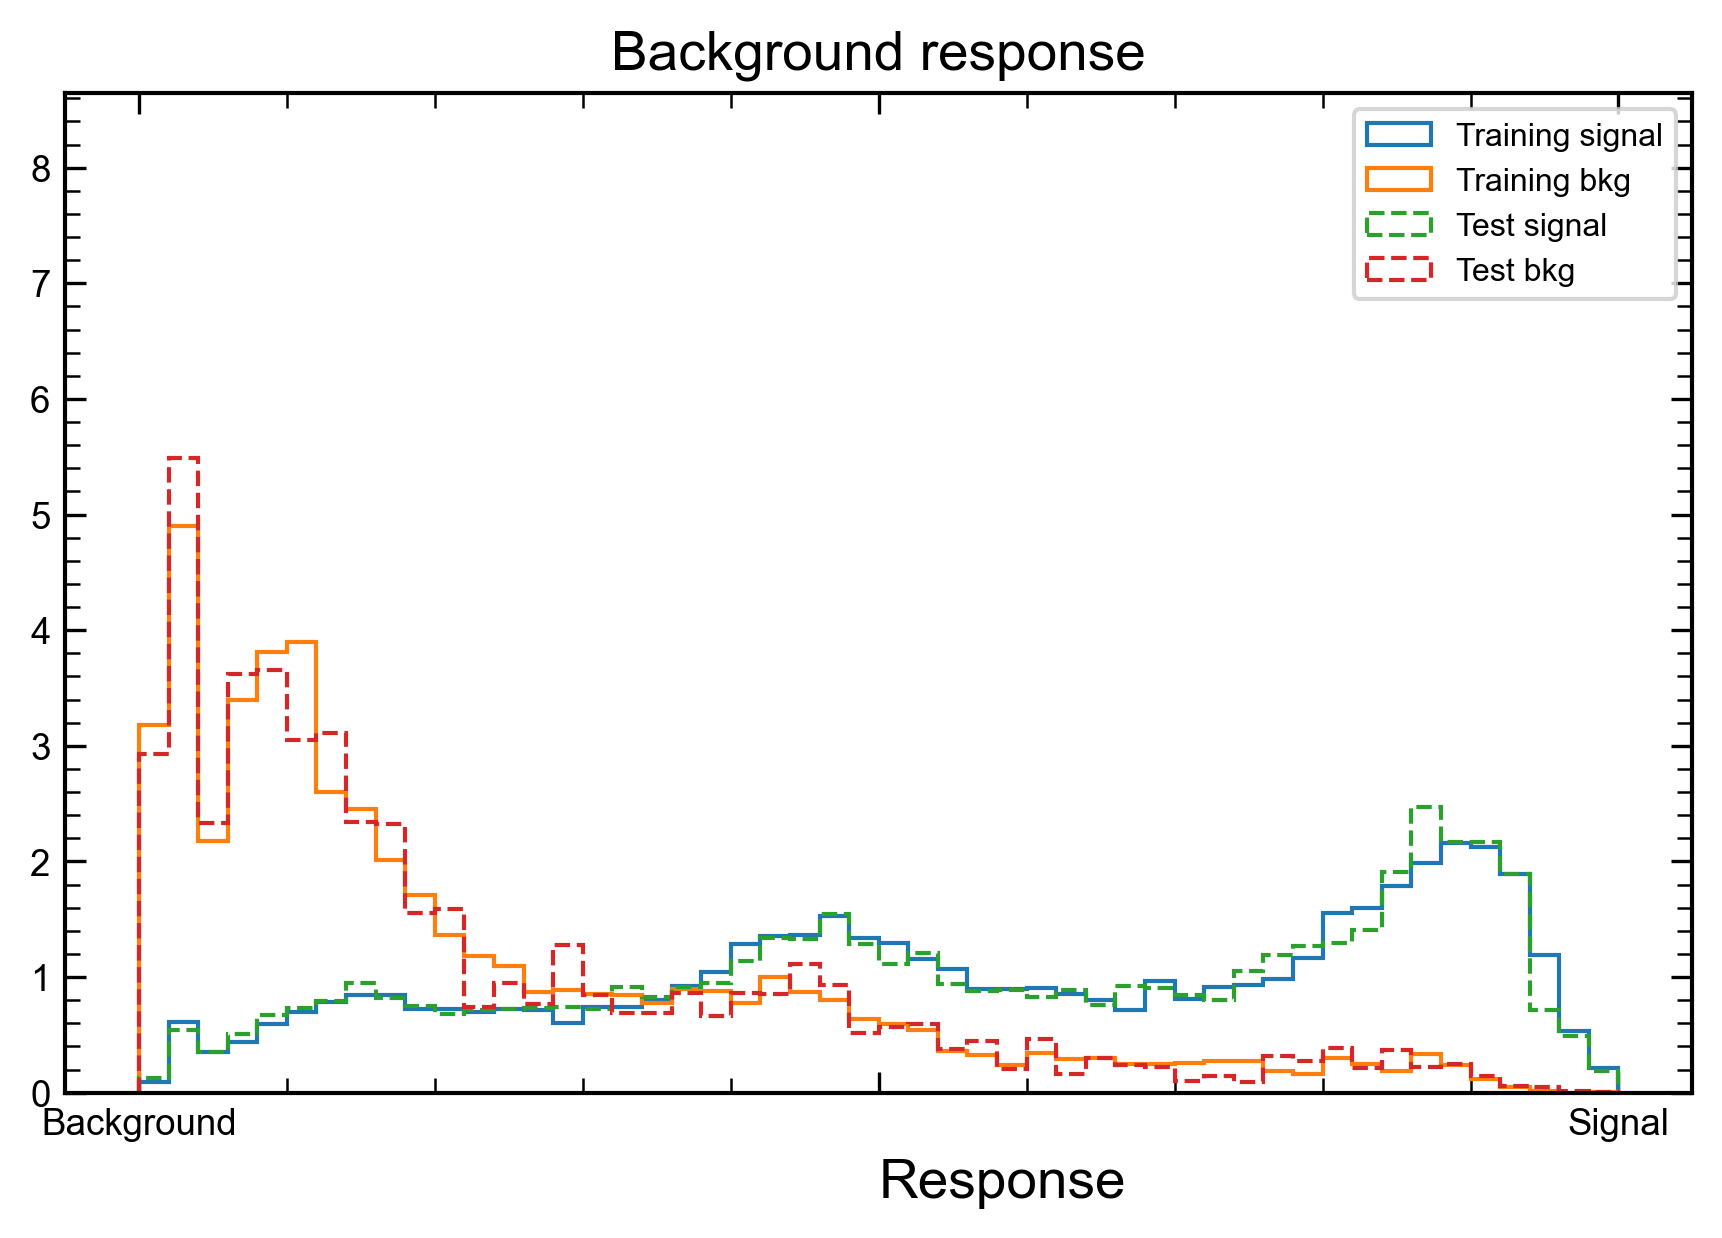
\includegraphics[width=0.8\textwidth]{bkg_lephad}
        \end{column}
        \begin{column}{0.5\textwidth}
            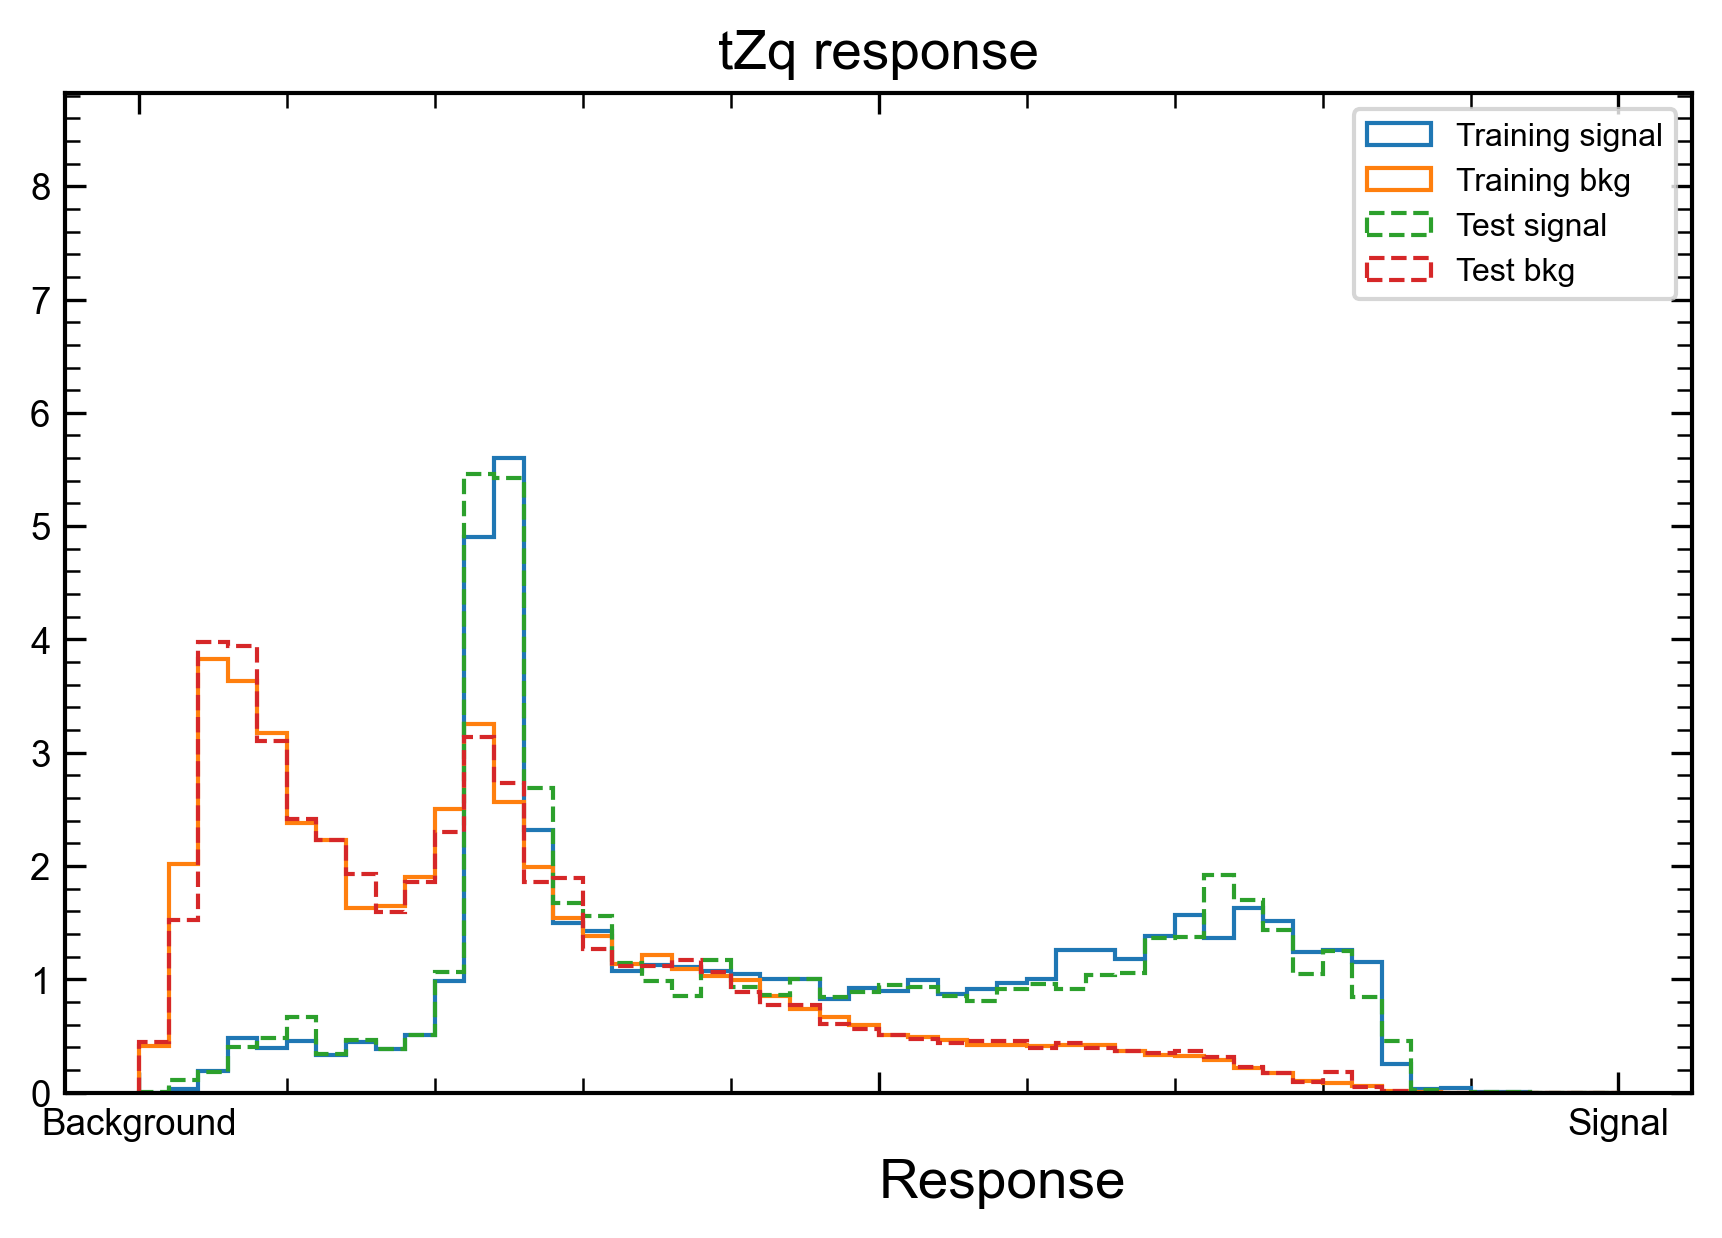
\includegraphics[width=0.8\textwidth]{tZq_lephad}
            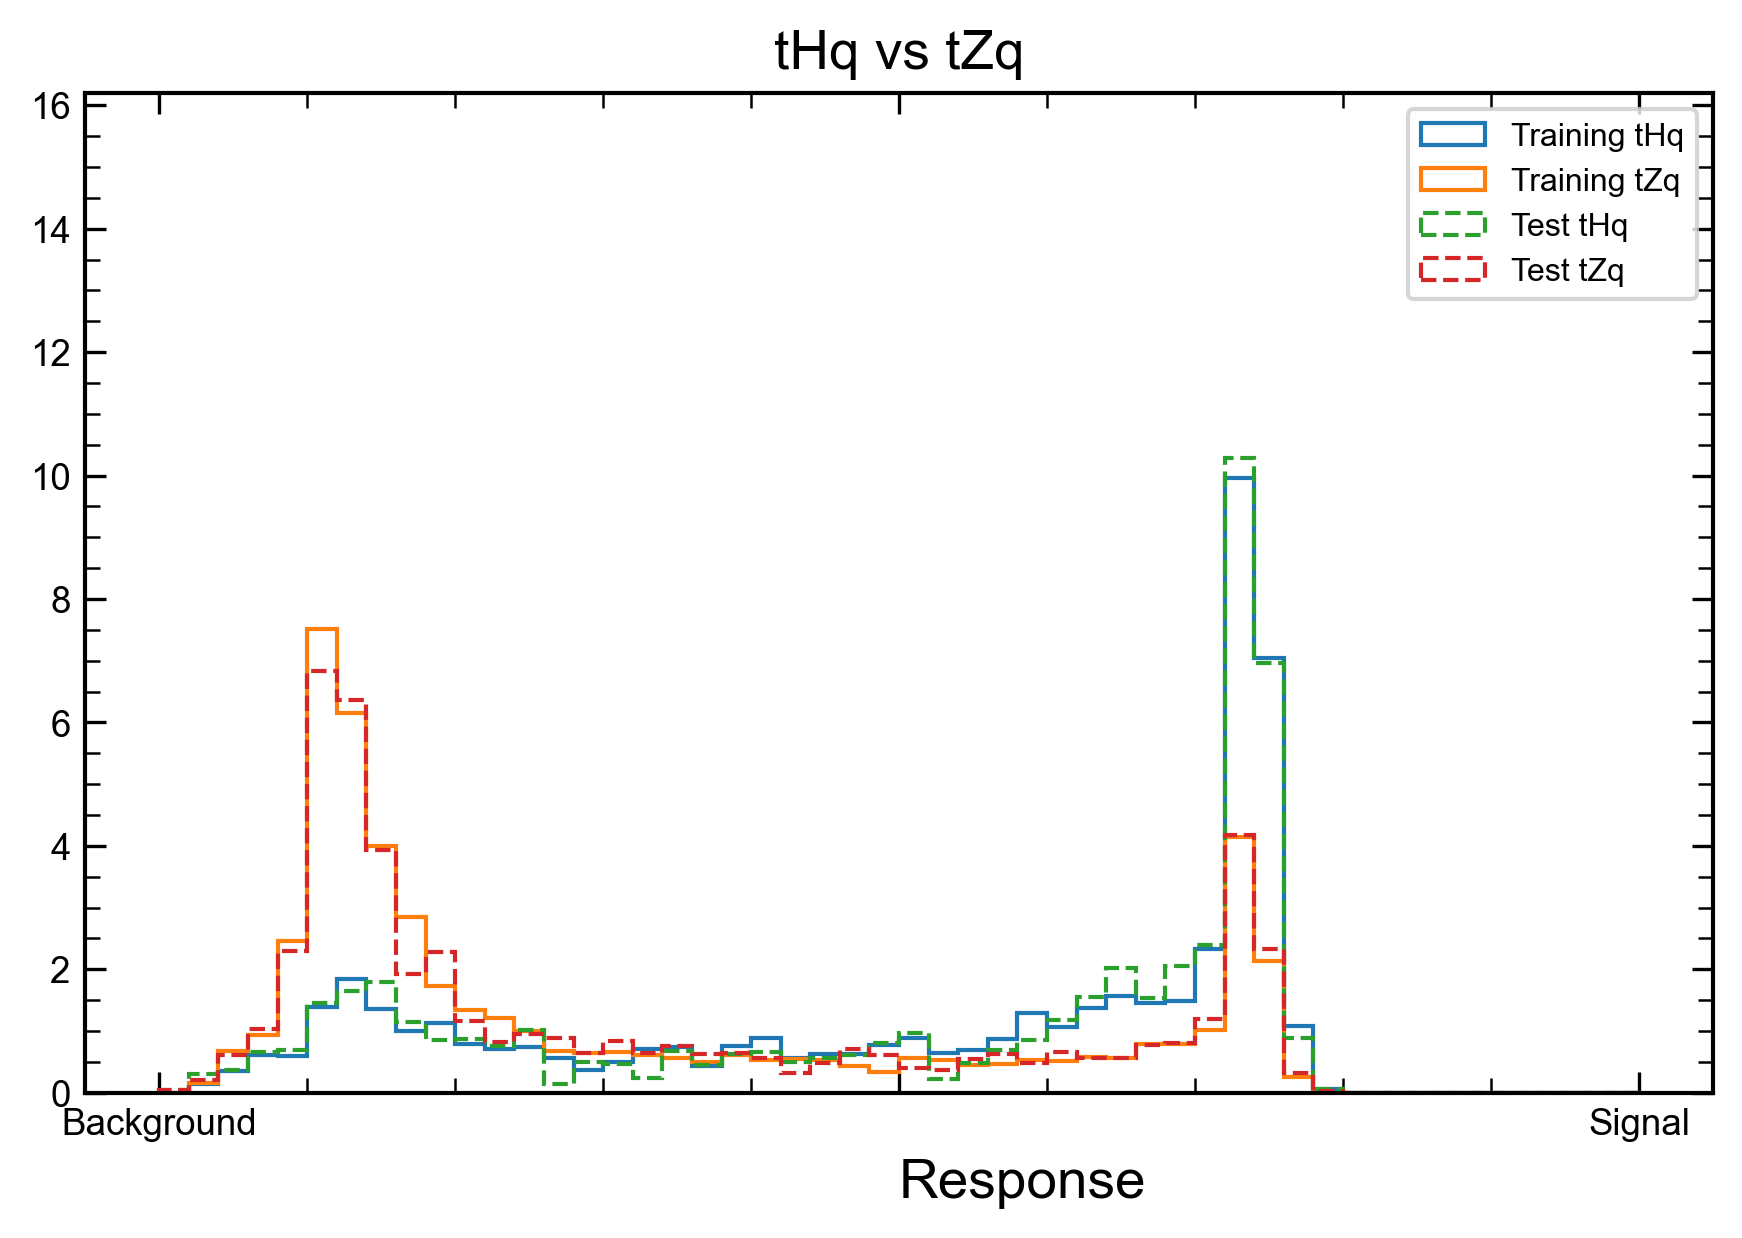
\includegraphics[width=0.8\textwidth]{comparison_lephad}
        \end{column}
    \end{columns}
\end{frame}

\begin{frame}{Yields}
    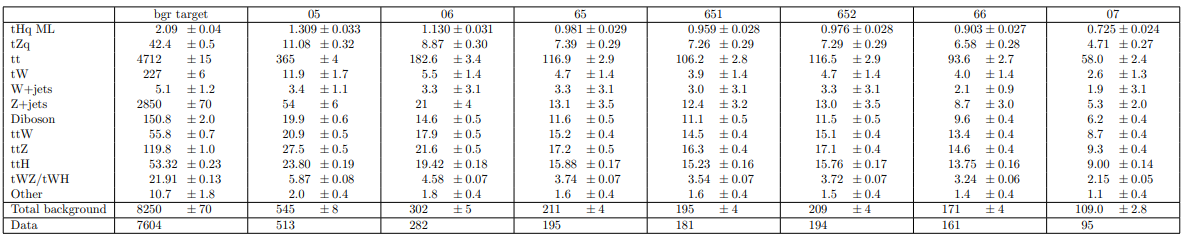
\includegraphics[width=\textwidth]{yields}
\end{frame}

\begin{frame}{S over B}
    \begin{columns}
        \begin{column}{0.5\textwidth}
            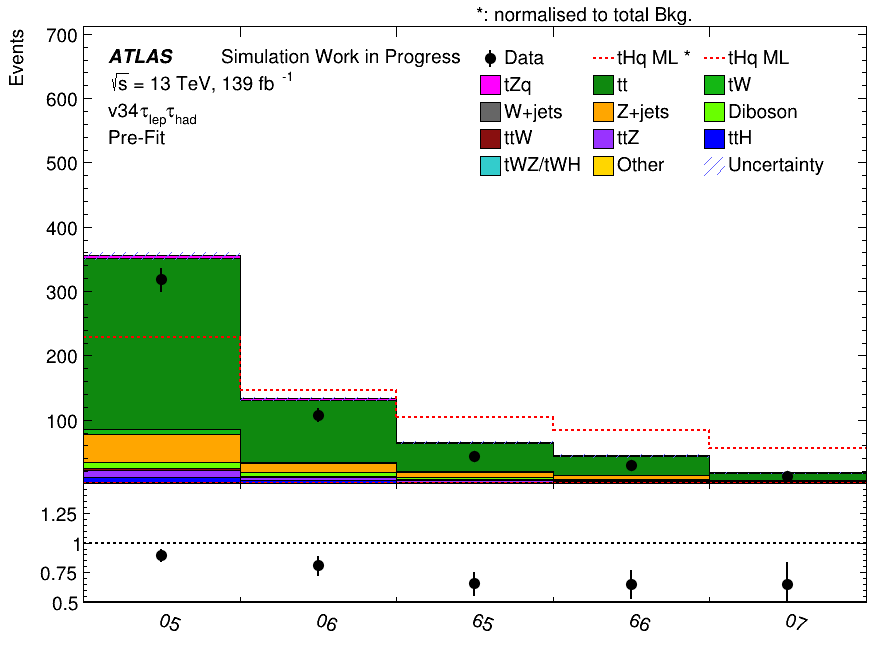
\includegraphics[width=0.8\textwidth]{Summary}
        \end{column}
        \begin{column}{0.5\textwidth}
            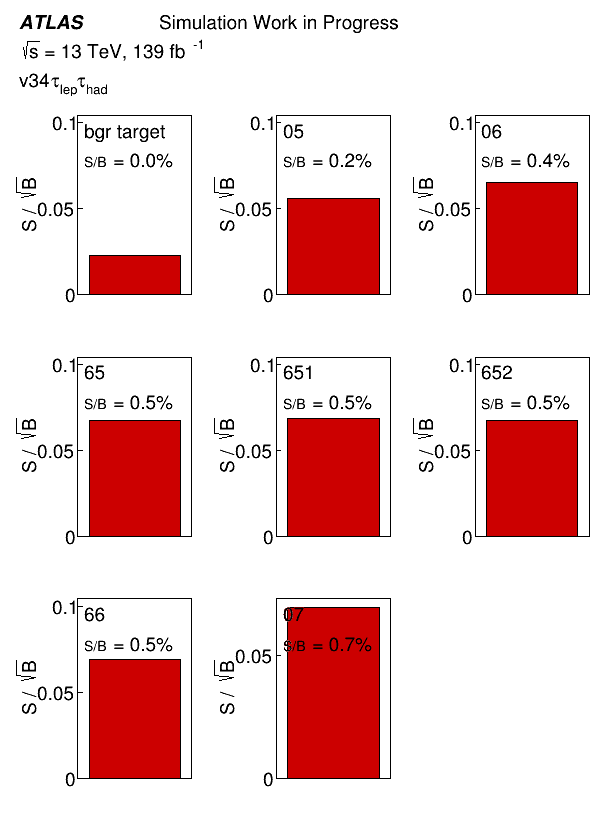
\includegraphics[width=0.8\textwidth]{soverb}
        \end{column}
    \end{columns}
\end{frame}

\begin{frame}{Summary}
    \begin{itemize}
        \item Every tool necessary to fit with the NN output is in place and tested 
        \item The model shows good stability and tests for negative weights setups hold
        \item Additionally, feature behaviour with respect wo weight sign was investigated
        \item Test fits created for lephad (and hadhad)
        \item Variable ranking planned, only needed for documentation
        \item Improved performance expected from combining categorical likelihhods, simple 2D cut not enough.
    \end{itemize}
\end{frame}



\begin{frame}{Summary}
\begin{table}[]
\begin{tabular}{|l|l|l|}
\hline
Feature                                             & Neural Network                   & BDT                             \\ \hline
AUC, positive weights only                          & -                                & 0.75                            \\ \hline
AUC                                                 & \cellcolor[HTML]{34FF34}0.82     & \cellcolor[HTML]{FE0000}0.52    \\ \hline
Feature optimisation                                & \cellcolor[HTML]{FE0000}not yet  & \cellcolor[HTML]{34FF34}done    \\ \hline
Evolutionary optimisation                           & \cellcolor[HTML]{34FF34}in place & \cellcolor[HTML]{34FF34}done    \\ \hline
Reduction of \tZq missclassification & \cellcolor[HTML]{34FF34}done     & -                               \\ \hline
Write response to tree                              & \cellcolor[HTML]{34FF34}done     & \cellcolor[HTML]{FE0000}not yet \\ \hline
\end{tabular}
\end{table}
\end{frame}

\section*{Backup}
\begin{frame}[plain,c]
%\frametitle{A first slide}

\begin{center}
\Huge Backup
\end{center}

\end{frame}

\begin{frame}{Evolutionary neural networks}
    \begin{itemize}
        \item Starting with a set of random configurations
        \vspace{0.2cm}
        \item Evaluate the results of the first generation and generate a new generation based on AUC 
        \vspace{0.2cm}
        \item Repeat until a good configuration is reached
        \vspace{0.2cm}
        \item Advantages:
            \begin{itemize}
                \item Decrease user bias for hyperparameter choice
                \item Optimised to run on worker nodes
                \item Quick discarding of bad configurations
                \item User friendly for unexperienced students
            \end{itemize}
    \end{itemize}
\end{frame}

%\begin{frame}{Inner product}
%    \begin{equation*}
%        a^{\mu} = \begin{pmatrix}
%            p_T \cosh ( \eta ) \\
%            p_T \cos ( \phi ) \\
%            p_T \sin ( \phi ) \\
%            p_T \sinh ( \eta ) \end{pmatrix}
%    \end{equation*}
%    %
%    \begin{align*}
%        \langle A | B \rangle = A_{\mu} B^{\mu}\\
%        = p_{T,A} p_{T,B} ( \cosh ( \eta_A ) \cosh ( \eta_B ) - \cos ( \phi_A ) \cos ( \phi_B)\\
%        - \sin ( \phi_A ) \sin ( \phi_B ) -\sinh ( \eta_A ) \sinh ( \eta_B ) )\\
%        = p_{T,A} p_{T,B} \left( \cosh ( \eta_A - \eta_B ) - \cos ( \phi_A - \phi_B ) \right)
%    \end{align*}
%\end{frame}

\begin{frame}{Responses}
  \begin{columns}
    \begin{column}{0.5\textwidth}
      \begin{figure}
      \centering 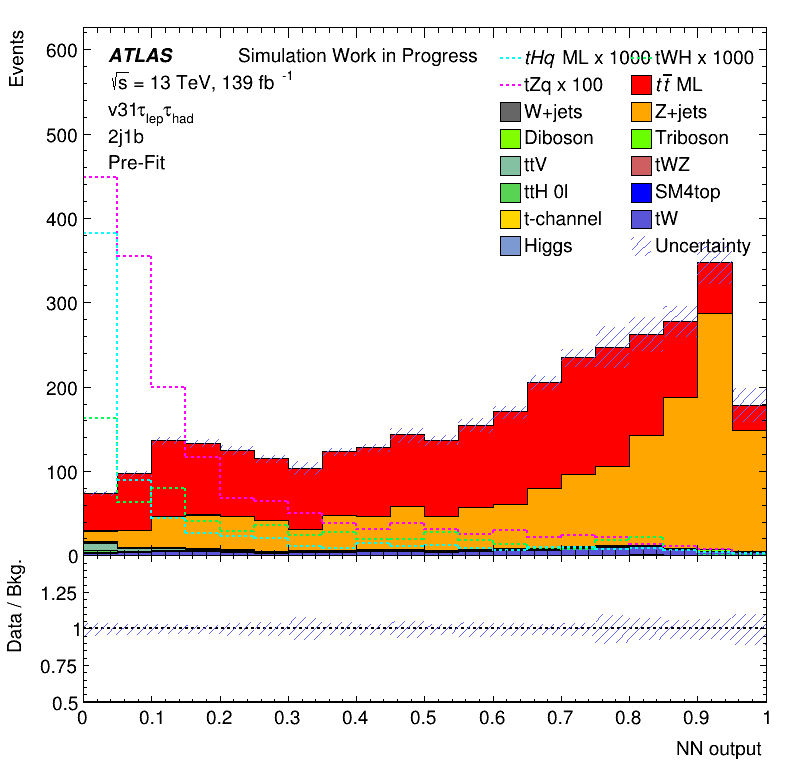
\includegraphics[width=\textwidth]{response_bkg}
      \caption{Background response}
      \end{figure}
    \end{column}
    \begin{column}{0.5\textwidth}
      \begin{figure}
      \centering 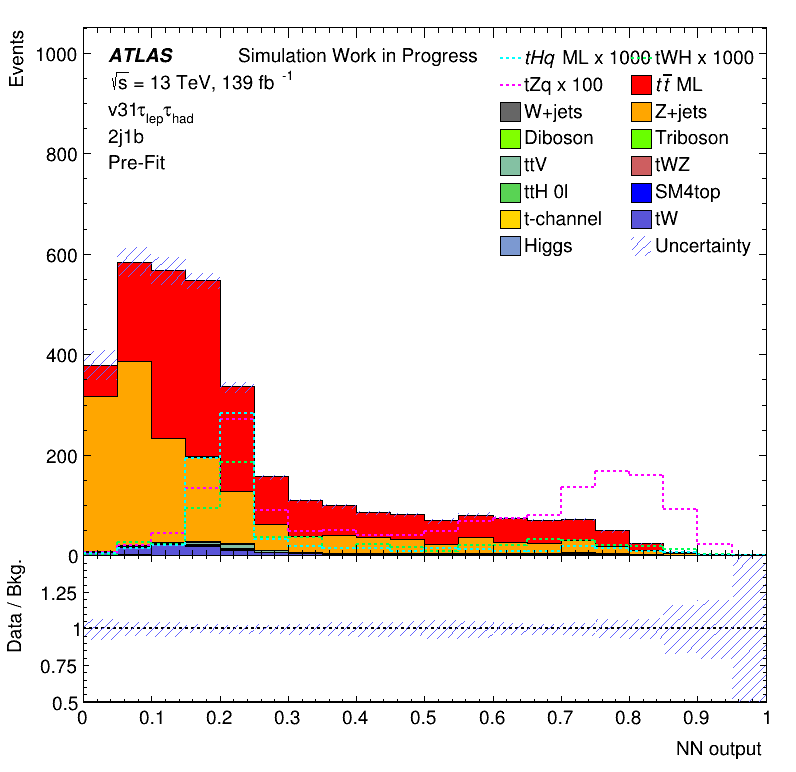
\includegraphics[width=\textwidth]{response_tZq}
      \caption{\tZq response}
      \end{figure}
    \end{column}
  \end{columns}
\end{frame}

\begin{frame}{\tHq versus \tZq}
  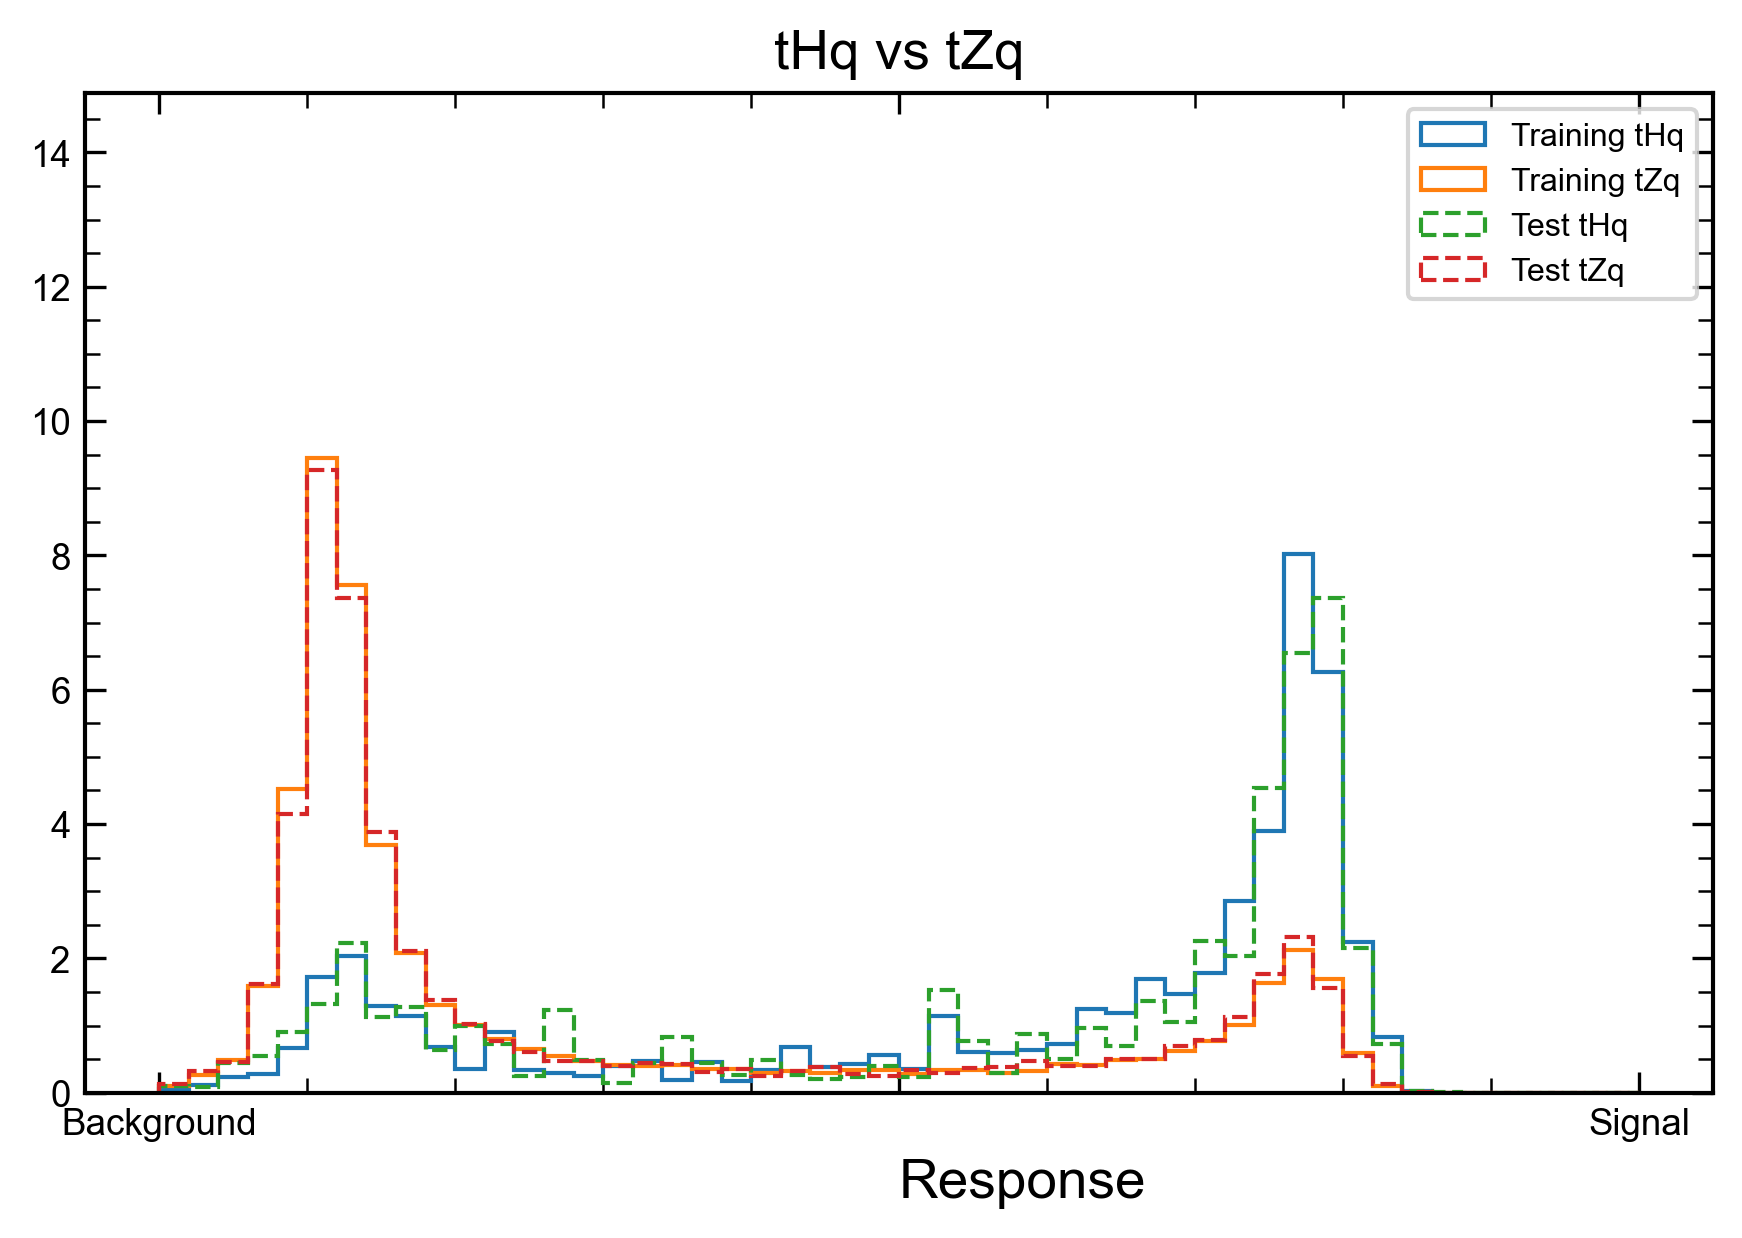
\includegraphics[width=\textwidth]{tHqvstZq.png}
\end{frame}

\begin{frame}{BDT summary}
    \begin{itemize}
        \item {\large A cut a bit below 0.2 would remove around 99\% of bkg
            events and 80\% of signal. Having just the 1\% of the bkg
            and 20\% of the signal would greatly increase our
            significance.}
        \vspace{0.2cm}
        \item {\large With the cut on the BDT we would have (approx.): bkg/sg = 4877/20 = 243
              Improved by a factor 71 to the before-presel scenario. Including BDT score in the trees}
        \vspace{0.2cm}
        \item {\large Using all events, not just the ones with positive weights reduces AUC surprisingly significantly}
        \vspace{0.2cm}
        \item {\large In the future the BDT should be tested in specific regions or for specific backgrounds}
    \end{itemize}
\end{frame}

\begin{frame}{}
  \centering 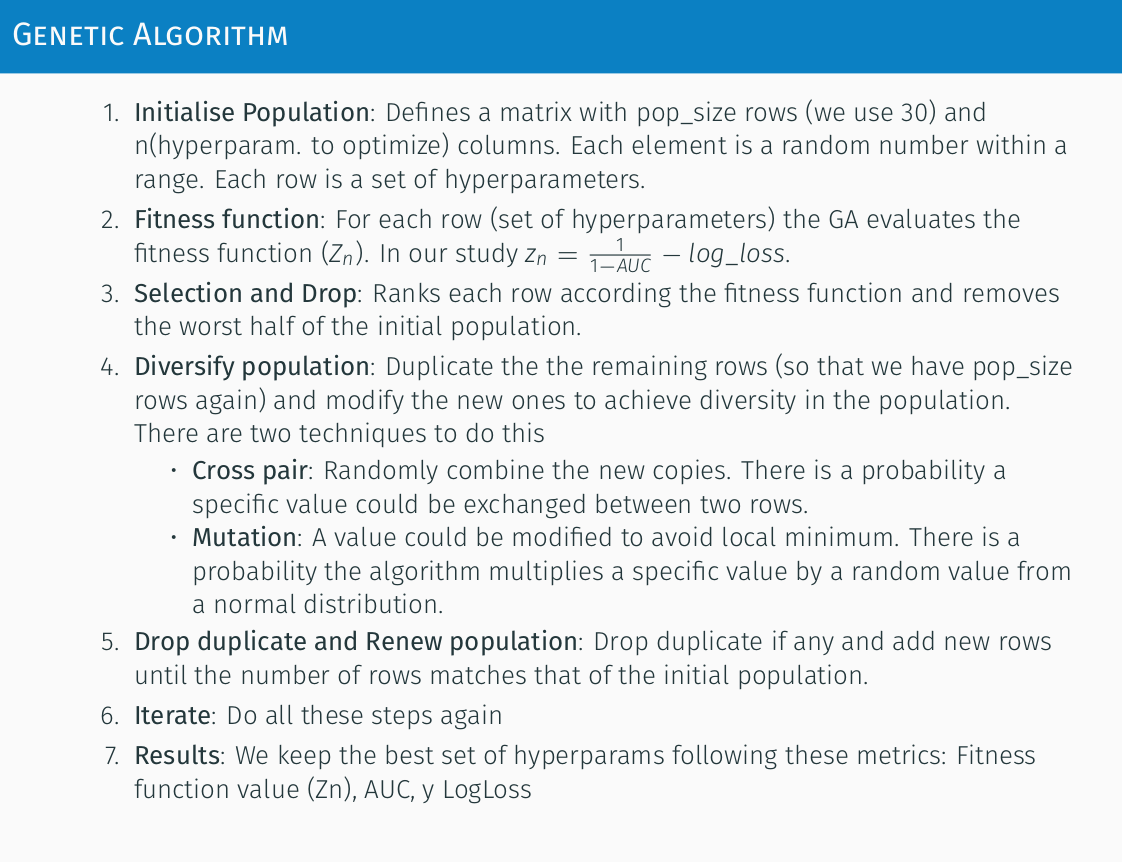
\includegraphics[width=\textwidth]{geneticAlg}
\end{frame}













\end{document}